\clearpage
\section{Plano de projeto}


\bigskip

\textbf{\ \ }\textcolor[rgb]{0.078431375,0.09411765,0.13725491}{Devido ao avanço tecnológico e a crescente necessidade
de encontrar soluções mais aprimoradas para o gerenciamento de um negócio, empresas buscam cada vez mais por sistemas
que auxiliem no controle e gestão de suas atividades.}

Esse projeto tem como objetivo a criação de um sistema para gerenciamento de restaurantes, permitindo o controle de
diversas funções como: estoque, atendimento e finanças. Esse sistema será integrado em computadores juntamente com o
uso de tecnologias móveis de forma a permitir uma maior eficiência tanto no atendimento ao cliente como no controle das
funções do restaurante. \ Devido a essa necessidade, além de computadores e uma rede de computadores, é necessário
também que o estabelecimento disponha de dispositivos móveis (tablets), para o uso nas atividades que exigem o
dispositivo.

O prazo necessário para conclusão das etapas de desenvolvimento e implantação do projeto foi estimado em 132 dias úteis.


\bigskip

\subsection{Problema}}


\bigskip

\textcolor[rgb]{0.078431375,0.09411765,0.13725491}{As atividades realizadas em um restaurante produzem uma grande
quantidade de informações como: pedidos de clientes, compras com fornecedores, contratação de funcionários e
gerenciamento de estoque. Devido a isso, surgem diversas dificuldades como: \ }

\liststyleWWNumi
\begin{itemize}
\item \textcolor[rgb]{0.078431375,0.09411765,0.13725491}{Gerência de grande volume de papel oriundo da venda de
refeições, da compra de itens com fornecedores e da administração de funcionários; }
\item \textcolor[rgb]{0.078431375,0.09411765,0.13725491}{Lentidão no atendimento aos clientes, sendo esta uma das
principais causas de cancelamento dos pedidos;}
\item \textcolor[rgb]{0.078431375,0.09411765,0.13725491}{Erros no preparo de pedidos dada a má compreensão do que é
anotado em comandas;}
\item \textcolor[rgb]{0.078431375,0.09411765,0.13725491}{Erros na entrega dos pedidos, onde é feita uma entrega em local
errado ou ainda o pedido não corresponde à solicitação desejada pelo cliente.}
\item \textcolor[rgb]{0.078431375,0.09411765,0.13725491}{Erros de cálculo quando a conta de uma comanda é solicitada;}
\end{itemize}

\bigskip


\bigskip

\clearpage
\subsection{Equipe}


\bigskip

\textcolor[rgb]{0.078431375,0.09411765,0.13725491}{A equipe é formada por um total
de}\textbf{\textcolor[rgb]{0.078431375,0.09411765,0.13725491}{ }}\textcolor[rgb]{0.078431375,0.09411765,0.13725491}{12
pessoas distribuídas entre as diferentes tarefas do sistema.}


\bigskip

\begin{flushleft}
\tablefirsthead{}
\tablehead{}
\tabletail{}
\tablelasttail{}
\begin{supertabular}{|m{5.302cm}|m{5.303cm}|m{5.2260003cm}|}
\hline
\centering \textbf{\textcolor[rgb]{0.078431375,0.09411765,0.13725491}{Profissional}} &
\centering \textbf{\textcolor[rgb]{0.078431375,0.09411765,0.13725491}{Quantidade}} &
\centering \textbf{\textcolor[rgb]{0.078431375,0.09411765,0.13725491}{Horas trabalhadas}}&\hline
\centering \textcolor[rgb]{0.078431375,0.09411765,0.13725491}{Administrador de Banco de Dados } &
\centering \textcolor[rgb]{0.078431375,0.09411765,0.13725491}{1} &
\centering\arraybslash \textcolor[rgb]{0.078431375,0.09411765,0.13725491}{264}& \hline
\centering \textcolor[rgb]{0.078431375,0.09411765,0.13725491}{Analista de Sistemas} &
\centering \textcolor[rgb]{0.078431375,0.09411765,0.13725491}{1} &
\centering\arraybslash \textcolor[rgb]{0.078431375,0.09411765,0.13725491}{688}& \hline
\centering \textcolor[rgb]{0.078431375,0.09411765,0.13725491}{Analista Programador Junior} &
\centering \textcolor[rgb]{0.078431375,0.09411765,0.13725491}{3} &
\centering\arraybslash \textcolor[rgb]{0.078431375,0.09411765,0.13725491}{480}& \hline
\centering \textcolor[rgb]{0.078431375,0.09411765,0.13725491}{Analista Programador Pleno} &
\centering \textcolor[rgb]{0.078431375,0.09411765,0.13725491}{3} &
\centering\arraybslash \textcolor[rgb]{0.078431375,0.09411765,0.13725491}{592}& \hline
\centering \textcolor[rgb]{0.078431375,0.09411765,0.13725491}{Analista Programador Sênior} &
\centering \textcolor[rgb]{0.078431375,0.09411765,0.13725491}{1} &
\centering\arraybslash \textcolor[rgb]{0.078431375,0.09411765,0.13725491}{592}& \hline
\centering \textcolor[rgb]{0.078431375,0.09411765,0.13725491}{Designer Pleno} &
\centering \textcolor[rgb]{0.078431375,0.09411765,0.13725491}{1} &
\centering\arraybslash \textcolor[rgb]{0.078431375,0.09411765,0.13725491}{200}& \hline
\centering \textcolor[rgb]{0.078431375,0.09411765,0.13725491}{Testador Pleno} &
\centering \textcolor[rgb]{0.078431375,0.09411765,0.13725491}{2} &
\centering\arraybslash \textcolor[rgb]{0.078431375,0.09411765,0.13725491}{248}& \hline
\end{supertabular}
\end{flushleft}

\bigskip


\bigskip


\bigskip

\clearpage
\subsection{Cronograma (Inclui Milestones)}


\bigskip

\begin{flushleft}
\tablefirsthead{}
\tablehead{}
\tabletail{}
\tablelasttail{}
\begin{supertabular}{|m{8.159cm}|m{2.8669999cm}|m{2.896cm}|m{1.813cm}|}
\hline
\centering \textbf{\textcolor[rgb]{0.078431375,0.09411765,0.13725491}{Nome}} &
\centering \textbf{\textcolor[rgb]{0.078431375,0.09411765,0.13725491}{Identificador}} &
\centering \textbf{\textcolor[rgb]{0.078431375,0.09411765,0.13725491}{Dependências}} &
\centering \textbf{\textcolor[rgb]{0.078431375,0.09411765,0.13725491}{Duração}}&
\hline
\textcolor[rgb]{0.078431375,0.09411765,0.13725491}{Levantamento de requisitos} &
\textcolor[rgb]{0.078431375,0.09411765,0.13725491}{T1} &
\textcolor[rgb]{0.078431375,0.09411765,0.13725491}{{}-} &
\textcolor[rgb]{0.078431375,0.09411765,0.13725491}{12 dias}\\\hline
\textcolor[rgb]{0.078431375,0.09411765,0.13725491}{Modelagem do software } &
\textcolor[rgb]{0.078431375,0.09411765,0.13725491}{T2} &
\textcolor[rgb]{0.078431375,0.09411765,0.13725491}{T1} &
\textcolor[rgb]{0.078431375,0.09411765,0.13725491}{15 dias}\\\hline
\textcolor[rgb]{0.078431375,0.09411765,0.13725491}{Modelagem BD} &
\textcolor[rgb]{0.078431375,0.09411765,0.13725491}{T3} &
\textcolor[rgb]{0.078431375,0.09411765,0.13725491}{T2} &
\textcolor[rgb]{0.078431375,0.09411765,0.13725491}{7 dias}\\\hline
\textcolor[rgb]{0.078431375,0.09411765,0.13725491}{Revisão dos requisitos} &
\textcolor[rgb]{0.078431375,0.09411765,0.13725491}{T4} &
\textcolor[rgb]{0.078431375,0.09411765,0.13725491}{T3} &
\textcolor[rgb]{0.078431375,0.09411765,0.13725491}{7 dias}\\\hline
\textcolor[rgb]{0.078431375,0.09411765,0.13725491}{Implementação do BD} &
\textcolor[rgb]{0.078431375,0.09411765,0.13725491}{T5} &
\textcolor[rgb]{0.078431375,0.09411765,0.13725491}{T3} &
\textcolor[rgb]{0.078431375,0.09411765,0.13725491}{7 dias}\\\hline
\textcolor[rgb]{0.078431375,0.09411765,0.13725491}{Desenvolvimento da interface gráfica} &
\textcolor[rgb]{0.078431375,0.09411765,0.13725491}{T6} &
\textcolor[rgb]{0.078431375,0.09411765,0.13725491}{T2} &
\textcolor[rgb]{0.078431375,0.09411765,0.13725491}{18 dias}\\\hline
\textcolor[rgb]{0.078431375,0.09411765,0.13725491}{Implementação de componentes auxiliares} &
\textcolor[rgb]{0.078431375,0.09411765,0.13725491}{T7} &
\textcolor[rgb]{0.078431375,0.09411765,0.13725491}{T2} &
\textcolor[rgb]{0.078431375,0.09411765,0.13725491}{7 dias}\\\hline
\textcolor[rgb]{0.078431375,0.09411765,0.13725491}{Implementação do Módulo Gerente} &
\textcolor[rgb]{0.078431375,0.09411765,0.13725491}{T8} &
\textcolor[rgb]{0.078431375,0.09411765,0.13725491}{T7} &
\textcolor[rgb]{0.078431375,0.09411765,0.13725491}{25 dias}\\\hline
\textcolor[rgb]{0.078431375,0.09411765,0.13725491}{Implementação do Módulo Garçom} &
\textcolor[rgb]{0.078431375,0.09411765,0.13725491}{T9} &
\textcolor[rgb]{0.078431375,0.09411765,0.13725491}{T7} &
\textcolor[rgb]{0.078431375,0.09411765,0.13725491}{18 dias}\\\hline
\textcolor[rgb]{0.078431375,0.09411765,0.13725491}{Implementação do Módulo do Estoquista} &
\textcolor[rgb]{0.078431375,0.09411765,0.13725491}{T10} &
\textcolor[rgb]{0.078431375,0.09411765,0.13725491}{T7} &
\textcolor[rgb]{0.078431375,0.09411765,0.13725491}{10 dias}\\\hline
\textcolor[rgb]{0.078431375,0.09411765,0.13725491}{Revisão de requisitos do módulo Gerente} &
\textcolor[rgb]{0.078431375,0.09411765,0.13725491}{T11} &
\textcolor[rgb]{0.078431375,0.09411765,0.13725491}{T8} &
\textcolor[rgb]{0.078431375,0.09411765,0.13725491}{10 dias}\\\hline
\textcolor[rgb]{0.078431375,0.09411765,0.13725491}{Revisão de requisitos do módulo Garçom} &
\textcolor[rgb]{0.078431375,0.09411765,0.13725491}{T12} &
\textcolor[rgb]{0.078431375,0.09411765,0.13725491}{T9} &
\textcolor[rgb]{0.078431375,0.09411765,0.13725491}{7 dias}\\\hline
\textcolor[rgb]{0.078431375,0.09411765,0.13725491}{Revisão de requisitos do módulo Estoquista} &
\textcolor[rgb]{0.078431375,0.09411765,0.13725491}{T13} &
\textcolor[rgb]{0.078431375,0.09411765,0.13725491}{T10} &
\textcolor[rgb]{0.078431375,0.09411765,0.13725491}{7 dias}\\\hline
\textcolor[rgb]{0.078431375,0.09411765,0.13725491}{Revisão de interface gráfica} &
\textcolor[rgb]{0.078431375,0.09411765,0.13725491}{T14} &
\textcolor[rgb]{0.078431375,0.09411765,0.13725491}{T11,T12,T13} &
\textcolor[rgb]{0.078431375,0.09411765,0.13725491}{7 dias}\\\hline
\textcolor[rgb]{0.078431375,0.09411765,0.13725491}{Teste \ do Módulo do Gerente} &
\textcolor[rgb]{0.078431375,0.09411765,0.13725491}{T15} &
\textcolor[rgb]{0.078431375,0.09411765,0.13725491}{T11} &
\textcolor[rgb]{0.078431375,0.09411765,0.13725491}{7 dias}\\\hline
\textcolor[rgb]{0.078431375,0.09411765,0.13725491}{Teste \ do Módulo do Garçom} &
\textcolor[rgb]{0.078431375,0.09411765,0.13725491}{T16} &
\textcolor[rgb]{0.078431375,0.09411765,0.13725491}{T12} &
\textcolor[rgb]{0.078431375,0.09411765,0.13725491}{7 dias}\\\hline
\textcolor[rgb]{0.078431375,0.09411765,0.13725491}{Teste \ do Módulo do Estoquista} &
\textcolor[rgb]{0.078431375,0.09411765,0.13725491}{T17} &
\textcolor[rgb]{0.078431375,0.09411765,0.13725491}{T13} &
\textcolor[rgb]{0.078431375,0.09411765,0.13725491}{7 dias}\\\hline
\textcolor[rgb]{0.078431375,0.09411765,0.13725491}{Geração de documentação do usuário} &
\textcolor[rgb]{0.078431375,0.09411765,0.13725491}{T18} &
\textcolor[rgb]{0.078431375,0.09411765,0.13725491}{T14} &
\textcolor[rgb]{0.078431375,0.09411765,0.13725491}{7 dias}\\\hline
\textcolor[rgb]{0.078431375,0.09411765,0.13725491}{Integração dos módulos} &
\textcolor[rgb]{0.078431375,0.09411765,0.13725491}{T19} &
\textcolor[rgb]{0.078431375,0.09411765,0.13725491}{T15,T16,T17} &
\textcolor[rgb]{0.078431375,0.09411765,0.13725491}{14 dias}\\\hline
\textcolor[rgb]{0.078431375,0.09411765,0.13725491}{Teste do sistema} &
\textcolor[rgb]{0.078431375,0.09411765,0.13725491}{T20} &
\textcolor[rgb]{0.078431375,0.09411765,0.13725491}{T19} &
\textcolor[rgb]{0.078431375,0.09411765,0.13725491}{10 dias}\\\hline
\textcolor[rgb]{0.078431375,0.09411765,0.13725491}{Implantação do sistema} &
\textcolor[rgb]{0.078431375,0.09411765,0.13725491}{T21} &
\textcolor[rgb]{0.078431375,0.09411765,0.13725491}{T20} &
\textcolor[rgb]{0.078431375,0.09411765,0.13725491}{14 dias}\\\hline
\end{supertabular}
\end{flushleft}

\bigskip

{\centering  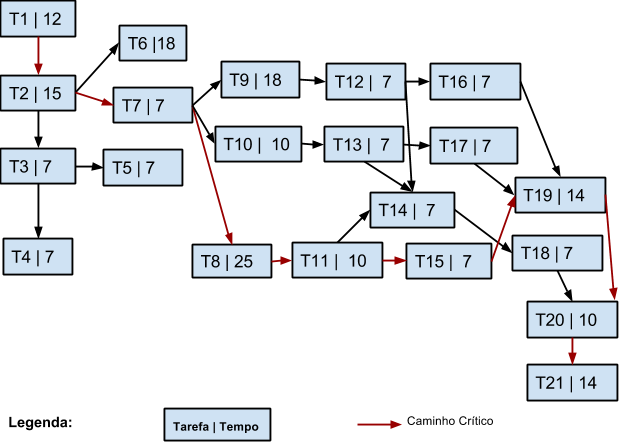
\includegraphics[width=16.722cm,height=11.834cm]{PlanodeProjeto-img002.png} \par}

\bigskip

A partir do caminho crítico mostrado, o tempo mínimo estimado para o projeto é 132 dias úteis.


\bigskip


\bigskip

\clearpage
\subsection{\textcolor[rgb]{0.078431375,0.09411765,0.13725491}{Estimativa de Custo}}\footnote{
\textcolor[rgb]{0.078431375,0.09411765,0.13725491}{O custo foi baseado nos valores disponíveis no seguinte endereço:
}\url{http://info.abril.com.br/noticias/carreira/2014/02/veja-o-salario-de-180-cargos-em-ti.shtml}\par }


\bigskip

\textbf{\textcolor[rgb]{0.078431375,0.09411765,0.13725491}{Custo com profissionais}}


\bigskip

\textcolor[rgb]{0.078431375,0.09411765,0.13725491}{O custo estimado com profissionais é mostrado e detalhado na tabela a
seguir.}


\bigskip


\bigskip

\begin{flushleft}
\tablefirsthead{}
\tablehead{}
\tabletail{}
\tablelasttail{}
\begin{supertabular}{|m{4.428cm}|m{3.476cm}|m{2.074cm}|m{2.4989998cm}|m{2.954cm}|}
\hline
\textbf{\textcolor[rgb]{0.078431375,0.09411765,0.13725491}{Profissional}} &
\textbf{\textcolor[rgb]{0.078431375,0.09411765,0.13725491}{Valor por hora Bruto (R\$)}} &
\textbf{\textcolor[rgb]{0.078431375,0.09411765,0.13725491}{Horas Mensais}} &
\textbf{\textcolor[rgb]{0.078431375,0.09411765,0.13725491}{Salário Mensal Bruto (R\$)}} &
\textbf{\textcolor[rgb]{0.078431375,0.09411765,0.13725491}{Salário Mensal Líquido (R\$)}}\\\hline
\textcolor[rgb]{0.078431375,0.09411765,0.13725491}{Administrador de Banco de Dados Pleno} &
\centering \textcolor[rgb]{0.078431375,0.09411765,0.13725491}{51,4046} &
\centering \textcolor[rgb]{0.078431375,0.09411765,0.13725491}{176} &
\centering \textcolor[rgb]{0.2,0.2,0.2}{9.047,21} &
\centering\arraybslash \textcolor[rgb]{0.2,0.2,0.2}{4.761,69}&\hline
\textcolor[rgb]{0.078431375,0.09411765,0.13725491}{Analista de Sistema Sênior} &
\centering \textcolor[rgb]{0.078431375,0.09411765,0.13725491}{62,0138} &
\centering \textcolor[rgb]{0.078431375,0.09411765,0.13725491}{176} &
\centering 10.914,43 &
\centering\arraybslash 5.744,44&\hline
\textcolor[rgb]{0.078431375,0.09411765,0.13725491}{Analista Programador Júnior} &
\centering \textcolor[rgb]{0.078431375,0.09411765,0.13725491}{26,1124} &
\centering \textcolor[rgb]{0.078431375,0.09411765,0.13725491}{176} &
\centering \textcolor[rgb]{0.2,0.2,0.2}{4.595,79} &
\centering\arraybslash \textcolor[rgb]{0.2,0.2,0.2}{2.418,84}&\hline
\textcolor[rgb]{0.078431375,0.09411765,0.13725491}{Analista Programador Pleno} &
\centering \textcolor[rgb]{0.078431375,0.09411765,0.13725491}{41,3600} &
\centering \textcolor[rgb]{0.078431375,0.09411765,0.13725491}{176} &
\centering \textcolor[rgb]{0.2,0.2,0.2}{7.279,37} &
\centering\arraybslash \textcolor[rgb]{0.2,0.2,0.2}{3.831,25}&\hline
\textcolor[rgb]{0.078431375,0.09411765,0.13725491}{Analista Programador Sênior} &
\centering \textcolor[rgb]{0.078431375,0.09411765,0.13725491}{58,1506} &
\centering \textcolor[rgb]{0.078431375,0.09411765,0.13725491}{176} &
\centering \textcolor[rgb]{0.2,0.2,0.2}{10.234,52} &
\centering\arraybslash \textcolor[rgb]{0.2,0.2,0.2}{5.386,59}&\hline
\textcolor[rgb]{0.078431375,0.09411765,0.13725491}{Designer Pleno} &
\centering \textcolor[rgb]{0.078431375,0.09411765,0.13725491}{21,6219} &
\centering \textcolor[rgb]{0.078431375,0.09411765,0.13725491}{176} &
\centering \textcolor[rgb]{0.2,0.2,0.2}{3.805,47} &
\centering\arraybslash \textcolor[rgb]{0.2,0.2,0.2}{2.002,88}&\hline
\textcolor[rgb]{0.078431375,0.09411765,0.13725491}{Testador Pleno} &
\centering \textcolor[rgb]{0.078431375,0.09411765,0.13725491}{32,7917} &
\centering \textcolor[rgb]{0.078431375,0.09411765,0.13725491}{176} &
\centering \textcolor[rgb]{0.2,0.2,0.2}{5.771,34} &
\centering\arraybslash \textcolor[rgb]{0.2,0.2,0.2}{3.037,55}&\hline
\end{supertabular}
\end{flushleft}
\liststyleWWNumii
\begin{itemize}
\item \textcolor[rgb]{0.078431375,0.09411765,0.13725491}{Assumindo que o valor dos impostos acumula 90\% sobre o salário
bruto de cada funcionário.}
\end{itemize}

\bigskip

\textbf{\textcolor[rgb]{0.078431375,0.09411765,0.13725491}{Custo com equipamento}}\footnote{ Valores dos
computadores retirados do site da Dell, Kabum, Saraiva}

\textcolor[rgb]{0.078431375,0.09411765,0.13725491}{O custo com equipamentos foi estimado de acordo com a quantidade de
produtos que serão comprados e os respectivos preços na data de escrita deste documento. Esse custo compreende os
seguintes equipamentos: 5 computadores de mesa, 5 computadores portáteis), 1 livro de banco de dados para consulta, 1
livro de programação mobile para consulta, 1}\textit{\textcolor[rgb]{0.078431375,0.09411765,0.13725491}{
tablet}}\textcolor[rgb]{0.078431375,0.09411765,0.13725491}{ para teste do módulo do garçom. Os valores desses
equipamentos são detalhados na tabela a seguir.}


\bigskip

\begin{flushleft}
\tablefirsthead{}
\tablehead{}
\tabletail{}
\tablelasttail{}
\begin{supertabular}{|m{4.984cm}|m{3.9799998cm}|m{2.7619998cm}|m{4.564cm}|}
\hline
\centering \textbf{\textcolor[rgb]{0.078431375,0.09411765,0.13725491}{Produto}} &
\centering \textbf{\textcolor[rgb]{0.078431375,0.09411765,0.13725491}{Valor unitário(R\$)}} &
\centering \textbf{\textcolor[rgb]{0.078431375,0.09411765,0.13725491}{Quantidade}} &
\centering\arraybslash \textbf{\textcolor[rgb]{0.078431375,0.09411765,0.13725491}{Custo (R\$)}}&\hline
\centering \textcolor[rgb]{0.078431375,0.09411765,0.13725491}{Computador de mesa} &
\centering \textcolor[rgb]{0.078431375,0.09411765,0.13725491}{1.500} &
\centering \textcolor[rgb]{0.078431375,0.09411765,0.13725491}{5} &
\centering\arraybslash \textcolor[rgb]{0.078431375,0.09411765,0.13725491}{7.500}&\hline
\centering \textcolor[rgb]{0.078431375,0.09411765,0.13725491}{Computador portátil} &
\centering \textcolor[rgb]{0.078431375,0.09411765,0.13725491}{1.600} &
\centering \textcolor[rgb]{0.078431375,0.09411765,0.13725491}{5} &
\centering\arraybslash \textcolor[rgb]{0.078431375,0.09411765,0.13725491}{8.000}&\hline
\centering \textcolor[rgb]{0.078431375,0.09411765,0.13725491}{Tablets} &
\centering \textcolor[rgb]{0.078431375,0.09411765,0.13725491}{800} &
\centering \textcolor[rgb]{0.078431375,0.09411765,0.13725491}{1} &
\centering\arraybslash \textcolor[rgb]{0.078431375,0.09411765,0.13725491}{800}&\hline
\centering \textcolor[rgb]{0.078431375,0.09411765,0.13725491}{Livros} &
\centering \textcolor[rgb]{0.078431375,0.09411765,0.13725491}{150} &
\centering \textcolor[rgb]{0.078431375,0.09411765,0.13725491}{2} &
\centering\arraybslash \textcolor[rgb]{0.078431375,0.09411765,0.13725491}{300}&\hline
\centering \textbf{\textcolor[rgb]{0.078431375,0.09411765,0.13725491}{Total}} &
\centering \textbf{\textcolor[rgb]{0.078431375,0.09411765,0.13725491}{4.050,00}} &
\centering \textbf{\textcolor[rgb]{0.078431375,0.09411765,0.13725491}{13}} &
\centering\arraybslash \textbf{\textcolor[rgb]{0.078431375,0.09411765,0.13725491}{16.600,00}}&\hline
\end{supertabular}
\end{flushleft}

\bigskip


\bigskip

\textbf{\textcolor[rgb]{0.078431375,0.09411765,0.13725491}{Custo com treinamento}}

\textcolor[rgb]{0.078431375,0.09411765,0.13725491}{Para adaptação dos programadores as tecnologias usadas no projeto, o
programador sênior fará um treinamento dos analistas programadores júnior durante a fase de levantamento de requisitos
e modelagem do projeto. Esse treinamento deve ser feito obrigatoriamente até o fim da tarefa 2 e somente haverá
treinamento dos profissionais de nível pleno, caso este profissional seja contratado sem passar pelo mesmo cargo de
nível júnior na empresa. Ou seja, não haverá custo extra com o treinamento já que esse profissional que fará o
treinamento estará recebendo o seu salário para essa função.}


\bigskip


\bigskip

\textbf{\textcolor[rgb]{0.078431375,0.09411765,0.13725491}{Custo com ambiente}}

\textcolor[rgb]{0.078431375,0.09411765,0.13725491}{Para o desenvolvimento do sistema, é necessária a aquisição ou
aluguel de um imóvel onde a equipe trabalhará. Foi estabelecido um valor de R\$ 900 mensais para o aluguel de uma sala
durante o tempo estimado no item 4, que foi de 132 dias. Com isso, o valor total estimado foi de R\$5.400,00.}


\bigskip

\textbf{\textcolor[rgb]{0.078431375,0.09411765,0.13725491}{Custo Total}}


\bigskip

\begin{flushleft}
\tablefirsthead{}
\tablehead{}
\tabletail{}
\tablelasttail{}
\begin{supertabular}{|m{13.213cm}|m{2.816cm}|}
\hline
\textbf{\textcolor[rgb]{0.078431375,0.09411765,0.13725491}{Tipo de custo}} &
\centering\arraybslash \textbf{\textcolor[rgb]{0.078431375,0.09411765,0.13725491}{\ Custo (R\$)}}&\hline
\textcolor[rgb]{0.078431375,0.09411765,0.13725491}{Custo com funcionários} &
\raggedleft\arraybslash \textcolor[rgb]{0.078431375,0.09411765,0.13725491}{222.307,7432}&\hline
\textcolor[rgb]{0.078431375,0.09411765,0.13725491}{Equipamentos} &
\raggedleft\arraybslash \textcolor[rgb]{0.078431375,0.09411765,0.13725491}{16.600,00}&\hline
\textcolor[rgb]{0.078431375,0.09411765,0.13725491}{Ambiente} &
\raggedleft\arraybslash \textcolor[rgb]{0.078431375,0.09411765,0.13725491}{5.400,00}&\hline
\textbf{\textcolor[rgb]{0.078431375,0.09411765,0.13725491}{Total}} &
\raggedleft\arraybslash \textbf{\textcolor[rgb]{0.078431375,0.09411765,0.13725491}{244.307,74}}&\hline
\end{supertabular}
\end{flushleft}

\bigskip
